\section{Plasticity model of EDZ}\label{sec:plasticity}





% \par In this section we assess the \gls{EDZ} at the \URFBII using the Hoek-Brown (\cite{hoek2019hoek}) empirical constitutive law within a FLAC3D numerical model.

% \subsection{Compilation of Damage Zones}
% According to \cite{Siren2015}, the concept of the Excavation Damaged Zone (EDZ) encompasses various sub-zones with distinct characteristics.
% % , see Fig. \ref{fig:damage_zones}
% These include:
% \begin{itemize}%[noitemsep]
%     \item \textbf{Stress-induced excavation damage zone (\Gls{EDZ}):} Zone of stress-induced irreversible damage, major property changes.
%     % \item \textbf{Construction induced excavation damage zone ($EDZ_C$):} Damage caused by construction method, significant property changes.
%     \item \textbf{Excavation influenced zone (\Gls{EIZ}):} Zone of stress-induced reversible changes, minor property changes.
%     \item \textbf{Blast-induced damage zone ($BIDZ$):} Zone of blast-induced irreversible fracturing, extremely significant property changes.
%     \item \textbf{Highly damaged zone ($HDZ$):} Excavation induced macro-scale fracturing or stress-induced spalling, significant property changes and instability.
% \end{itemize}

% \begin{figure}%[H]
%     \centering
%     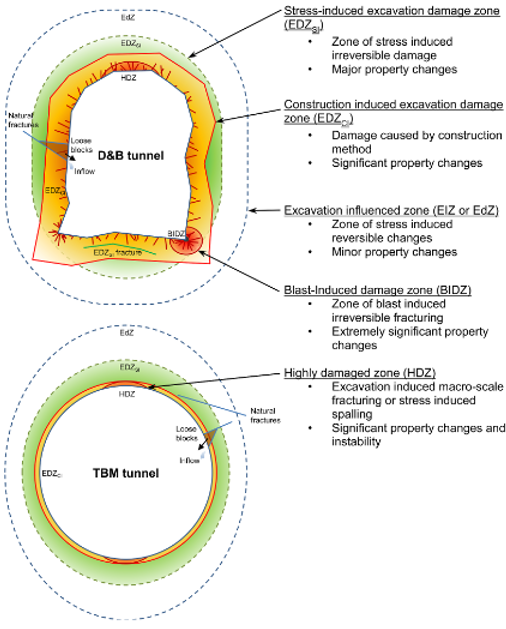
\includegraphics[width=0.5\textwidth]{graphics/plasticity/damage_zones.png} % Example image path
%     \caption{Compilation of damage zones with their definitions in a generic stress field (Siren, 2015).}
%     \label{fig:damage_zones}
% \end{figure}
% \newpage


% \sts{[S: Nize uvedene tri odstavce se nehodi do uvodu - mely by byt premisteny na vhodnejsi mista nebo odstraneny.]}

% \par The study focuses on characterizing the rock mass behavior under excavation conditions, considering the specific geological context and the influence of pore water pressure (PWP). Although a detailed geological model of the site was constructed, for this analysis, the rock mass was simplified to a single Hoek-Brown material with properties $E$ = 72.5 GPa, $\nu$ = 0.215, and $UCS$ = 170.3 MPa.

% \par The simulation was performed in a staggered approach to accurately model the excavation process. For each sequential excavation stage, time-dependent pore water pressure data—obtained from a fully-coupled poroelastic model developed by \gls{TUL} researchers—was imported. This methodology ensured that the PWP field within the model was synchronized with both the excavation advance  in the test chambers ZK5-1S and ZK5-1J.

% \par The results indicate that the \gls{EDZ} is predominantly located in the walls of the excavation rather than the roofs. The estimated extent of the \gls{EDZ} is between 0.5 to 1 meter, a range that is constrained by the resolution of the chosen numerical mesh.

% \newpage

% \section*{List of Abbreviations}
% \begin{tabularx}{\textwidth}{@{}lX@{}} % The @{} removes padding
% \textbf{Abbreviation} & \textbf{Description} \\
% \midrule
% BIDZ & Blast-Induced Damage Zone \\
% D & Disturbance Factor \\
% DGR & Deep Geological Repository \\
% E & Young's Modulus \\
% EDZ & Excavation Damaged Zone \\
% $EDZ_{C}$ & Construction Induced Excavation Damage Zone \\
% $EDZ_{EI}$ & Excavation Influenced Zone \\
% $EDZ_{SI}$ & Stress-Induced Excavation Damage Zone \\
% EIZ & Excavation Influenced Zone \\
% FLAC3D & Fast Lagrangian Analysis of Continua in 3 Dimensions \\
% IGN & Institute of Geonics \\
% GPa & Gigapascals \\
% GSI & Geological Strength Index \\
% HDZ & Highly Damaged Zone \\
% $m_b$ & Hoek-Brown Rock Mass Parameter \\
% $m_i$ & Hoek-Brown Intact Rock Parameter \\
% MPa & Megapascals \\
% PWP & Pore Water Pressure \\
% $s$ & Hoek-Brown Rock Mass Parameter \\
% $S_H$ & Maximum Horizontal Stress \\
% $S_h$ & Minimum Horizontal Stress \\
% $S_v$ & Vertical Stress \\
% TUL & Technical University of Liberec \\
% UCS & Uniaxial Compressive Strength \\
% URF & Underground Research Facility \\
% $\nu$ & Poisson's Ratio \\
% \bottomrule
% \end{tabularx}



% \subsection{Introduction}

% Estimating the extent of \gls{EDZ} in underground structures, such as the BUKOV URF, is critical for evaluating structural integrity and safety. The extent of the \gls{EDZ} in the presence of water is governed by a complex interplay of hydraulic and mechanical interactions.

% \par In countries like the Czech Republic, where \gls{DGR} for radioactive waste are planned in brittle crystalline rocks with fractures at various scales, understanding these processes becomes even more crucial.

This section summarizes the assessment of \gls{EDZ} at the \URFBII, with a specific focus on the excavation of corridors ZK5-1S and ZK5-1J in the L5 gallery. We use the Hoek-Brown empirical constitutive law \eqref{eq:hoek-brown}, see \cite{hoek2019hoek}, within a FLAC3D numerical model (referred to as \textbf{Model 2}) to characterize the rock mass behavior under excavation conditions, considering the specific geological context and the influence of \Gls{PWP}.

% \sts{[S: Nize uvedeny odstavec se nehodi do uvodu - mely by byt premisteny na vhodnejsi misto a mel by byt uveden odkaz na treti kapitolu.]}



% \begin{figure}%[H]
%     \centering
%     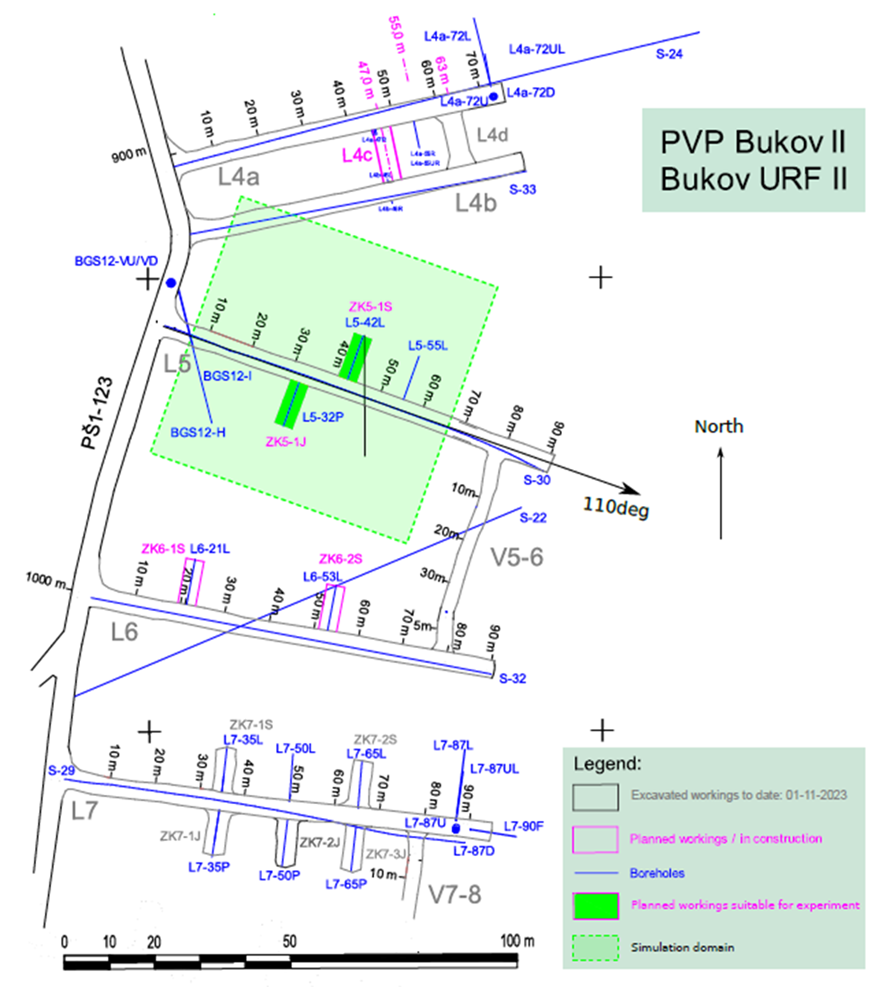
\includegraphics[width=0.8\textwidth]{graphics/plasticity/modeling_ext.png}
%     \caption{PVP Bukov II URF. Simulation domain in green. Source: Chodby, 2024}
%     \label{fig:modeling_ext}
% \end{figure}

 
\subsection{Proposed methodology}

In order to take the effect of \Gls{PWP} into account in the assessment of \Gls{EDZ}, we import the pressure field from the fully coupled poroelastic simulation (Model 1), described in Sec. \ref{sec:model_comparison}, to the FLAC3D plasticity simulation (Model 2).

The main steps of the analysis of the extent of \Gls{EDZ} are as follows.

\begin{enumerate}
\item \textbf{Geological and Geomechanical Characterization:} Characterize the lithologies within the model domain to establish appropriate Hoek-Brown parameters. These properties are derived by fitting the results from triaxial laboratory testing.
\item \textbf{\gls{PWP} Field Generation:} Import and interpolate the \gls{PWP} field into the FLAC3D model. This imported data will serve as the initial condition for each sequential excavation stage. 
\item \textbf{Numerical Model Construction:} Construct the numerical model by meshing the geological domain and assigning the derived Hoek-Brown parameters to the respective lithologies.
\item \textbf{EDZ Assessment:} Evaluate the extent and shape of the \gls{EDZ} by analyzing the yielded zones and associated rock mass strains.
\end{enumerate}

% Na tabulku se nikde v textu neodkazuje - zakomentovano.
% \begin{table}%[H]
%     \centering
%     \caption{Summary of outcomes from different EDZ assessments.}
%     \label{tab:edz_approaches}
%     \begin{tabularx}{\textwidth}{lXX} % Changed to tabularx with X columns
%         \toprule
%         \textbf{Aspect} & \textbf{Steady-State Pore Pressure} & \textbf{Re-Adjusted Pore Pressure}\newline\textbf{(Fully coupled or staged analysis)} \\ % Added \newline
%         \midrule
%         \textbf{EDZ Extent} & Potentially over/underestimated & More localized or extensive based on dissipation \\
%         \textbf{EDZ Shape} & More uniform, symmetric & Asymmetric, influenced by drainage paths \\
%         \textbf{Deformation} & Over/underestimated & Dynamic, accounting for drainage \\
%         \textbf{Effective Stress} & Static, unrealistic in places & Evolves dynamically with pore pressures \\
%         \textbf{Hydraulic Feedback} & Ignored & Fully considered \\
%         \bottomrule
%     \end{tabularx}
% \end{table}

\paragraph{Common approaches for EDZ estimation.}
Different approaches exist for estimating the \gls{EDZ} extent, each with its strengths and weaknesses, particularly concerning the treatment of pore pressure. Assuming a steady-state pore pressure throughout the simulation can have drawbacks, leading to potentially over/underestimated \gls{EDZ} extents and more uniform shapes. Fully coupled simulations, while more accurate, are time-demanding. Staged analysis, where a pure hydro simulation is performed after each significant mechanical stage, allows for changes in hydraulic properties due to damaged zones, inducing new water pathways and higher pore water pressure in these areas.
% The paper by \cite{Marschall2017} is particularly rich in these insights.
For details on the comparison of the methods we refer to the paper by \cite{Marschall2017}.

\paragraph{Geometry and mesh generation.}
The numerical model's geometry and the progressive excavation stages are central to this study.
It is assumed that the test chambers ZK5-1S and ZK5-1J were excavated in distinct stages over time, as detailed in Table \ref{tab:excavation_advances} (see also Fig. \ref{fig:excavation_progress}), to realistically simulate the rock's response.

The model geometry is based on an initial tunnel scan, which was softened using Rhino commands (e.g., QuadRemesh) to achieve a 'noise-free' mesh. 
\par The mesh was adjusted to the mesh of Model 1 to avoid large discrepancies in coordinates, and so that the location of the box and tunnels are consistent with mesh of Model 1.
\begin{itemize}%[noitemsep]
    \item \textbf{Hexa-dominated mesh:} This is the mesh of Model 2. Size of approximately 0.2-0.5 m around tunnels and 1 m in the outer box.
    \item \textbf{Tetra mesh:} This is the mesh of Model 1. Size of approximately 0.8 m around tunnels and approximately 12 m in the outer box.
\end{itemize}


To simulate the mechanical excavation as realistically as possible, the mesh for the test chambers ZK5-1S and ZK5-1J was incrementally cut at specific time-based intervals. The distances between these successive cuts and their corresponding time events --- referenced from the fully-coupled poroelastic Model 1 --- are detailed in Table~\ref{tab:excavation_advances}. This process ensured that the pore water pressure import into FLAC3D was precisely synchronized with each excavation stage.

\begin{table}%[H]
    \centering
    \caption{Excavation advances for ZK5-1S and ZK5-1J.}
    \label{tab:excavation_advances}
    \begin{tabular}{cccc}
        \toprule
        Time [days] & $d_{ZK5-1S}$ [m] & Time [days] & $d_{ZK5-1J}$ [m] \\
        \midrule
        0 & 0 & 0 & 0 \\
        101.667 & 1.8 & 112.01 & 1.6 \\
        103.434 & 3.6 & 115.688 & 3.5 \\
        104.66 & 5.8 & 117.684 & 5.5 \\
        107.667 & 7.1 & 123.438 & 7.2 \\
        108.667 & 8.5 & 125.385 & 9.3 \\
        110.379 & 11 & 129.358 & 11 \\
        \bottomrule
    \end{tabular}
\end{table}

FLAC3D mesh incorporates the mechanical advance cuts and the intersections of the aforementioned cuts with the complex geology elaborated. 

\begin{figure}%[H]
    \centering
    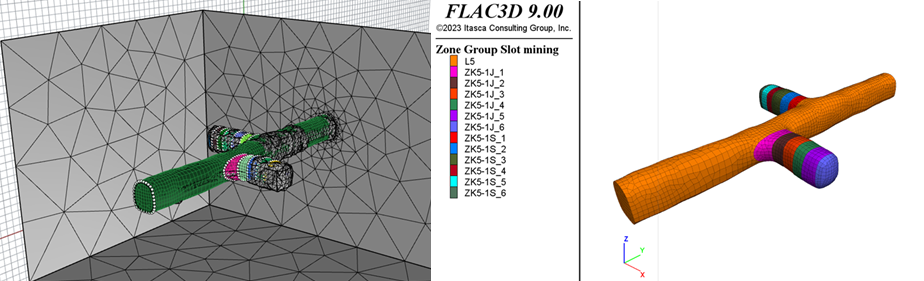
\includegraphics[width=0.9\textwidth]{graphics/plasticity/mesh_comparison.png} % Example image path
    \caption{Comparison between mesh of Model 1 and Model 2, showing the matched geometry.}
    \label{fig:mesh_comparison}
\end{figure}
% \footnotetext{\gls{TUL} mesh is basically the mesh in which pore water pressure was originally computed as an output.}

\paragraph{Physical parameters and boundary conditions.}
The model parameters are taken in accordance with Chapter \ref{chapter:review} and Section \ref{sec:model_comparison}.
In particular, the Hoek-Brown parameters are determined in Section \ref{sec:review_mech}.

Although the geology of the site is much more complicated, here a single Hoek-Brown material has been considered with properties $E = 72.5 \munit{GPa}$, $\nu = 0.215$, and $UCS = 170.3 \munit{MPa}$, which correspond to the fitted parameters of amphibolite, Section \ref{sec:review_mech}, whose presence is significant around the modeled tunnels.


% \newpage

% \paragraph{Boundary Conditions.}

% \sts{[S: Nize uvedene hodnoty je treba dat do souvislosti se treti kapitolou, pripadne kapitolu 3 doplnit.]}

The initial stress state is defined as in Model 1, namely by:
\begin{itemize}%[noitemsep]
    \item Maximum horizontal stress ($S_H$) = $-42$ \unit\MPa;
    \item Minimum horizontal stress ($S_h$) = $-19$ \unit\MPa;
    \item Vertical stress ($S_v$) = $-14$ \unit\MPa.
\end{itemize}
Here the values are negative for compressive stresses, in agreement with FLAC3D convention.
The azimuth of $S_H$ is $123^\circ$ clockwise from North ($13^\circ$ from L5 axis).
% The vertical stress is -14 MPa.
Stresses are initialized by means of a given stress tensor.
% It is worth mentioning that, according to FLAC's convention, the negative sign in stresses indicates compressive regime. 

\begin{figure}%[H]
    \centering
    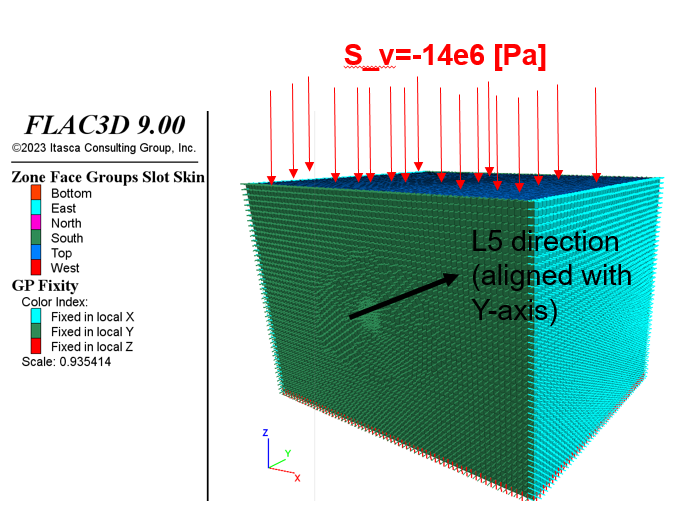
\includegraphics[width=0.9\textwidth]{graphics/plasticity/boundary_conditions.png} % Example image path
    \caption{FLAC3D model showing the applied boundary conditions and initial stress field.}
    \label{fig:boundary_conditions}
\end{figure}

This gives a horizontal-to-vertical stress ratio $\sigma_H/\sigma_v=3$, corresponding to a highly anisotropic stress field and a known driver of extensional failure in underground excavation walls (\cite{Barton2017}).

% \newpage
\subsection{Stages of modeling}

The modeling process follows a staged approach, where the initial stage %(day 100\_dry.f3sav) 
assumes L5 is already excavated. Subsequent stages involve mechanical advances followed by \gls{PWP} updates, reflecting a dry-to-wet transition.

The \gls{PWP} is imported into FLAC3D at each update as an input, for effective stress calculation (\cite{Brace1968}).


The excavation advances for ZK5-1S and ZK5-1J are applied incrementally, with \gls{PWP} contours updated at each stage. For instance, in Update 1, the \gls{PWP} of 101.667 days is applied. This logic is applied for subsequent excavations.
Thus, according to \autoref{tab:excavation_advances}, the model considers 6 stages/updates for ZK5-1S and ZK5-1J.  The final update, 'update13' represents a period of relaxation of 10 years.

\subsection{Results: EDZ contours}
The extent of the \gls{EDZ} is visualized through yielded zones, specifically using \textquote{Zone State By Any} and \textquote{Zone State By Average} criteria in FLAC3D. A cut plane at $z=2$ \unit\meter~ (dip/dipdir = 180/180) is used for standardized visualization.
\begin{itemize}%[noitemsep]
    \item \textbf{Zone State By Any:} This method is very sensitive to the initiation of yielding. As soon as the most highly stressed point within a zone yields, the whole zone gets colored.
    \item \textbf{Zone State By Average:} This method colors a zone according to a yield state only if that state is predominant or representative among the internal calculation points. For instance, it might require a majority of points to be yielded, or it might perform some form of weighted averaging.
\end{itemize}



\begin{figure}%[H]
    \centering
    \begin{subfigure}[b]{0.48\textwidth}
        \centering
        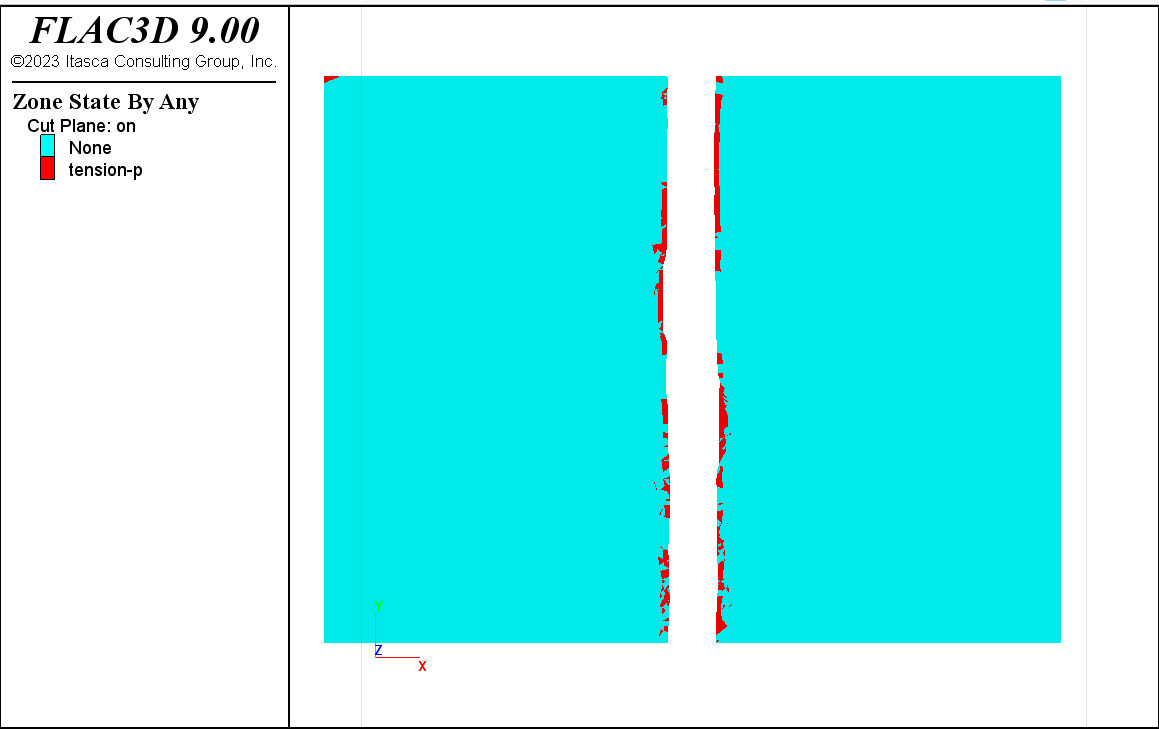
\includegraphics[width=\textwidth]{graphics/plasticity/update0.png}
        \caption{Update 0}
        \label{fig:zk5_1s_mosaic_0}
    \end{subfigure}
    \hfill
    \begin{subfigure}[b]{0.48\textwidth}
        \centering
        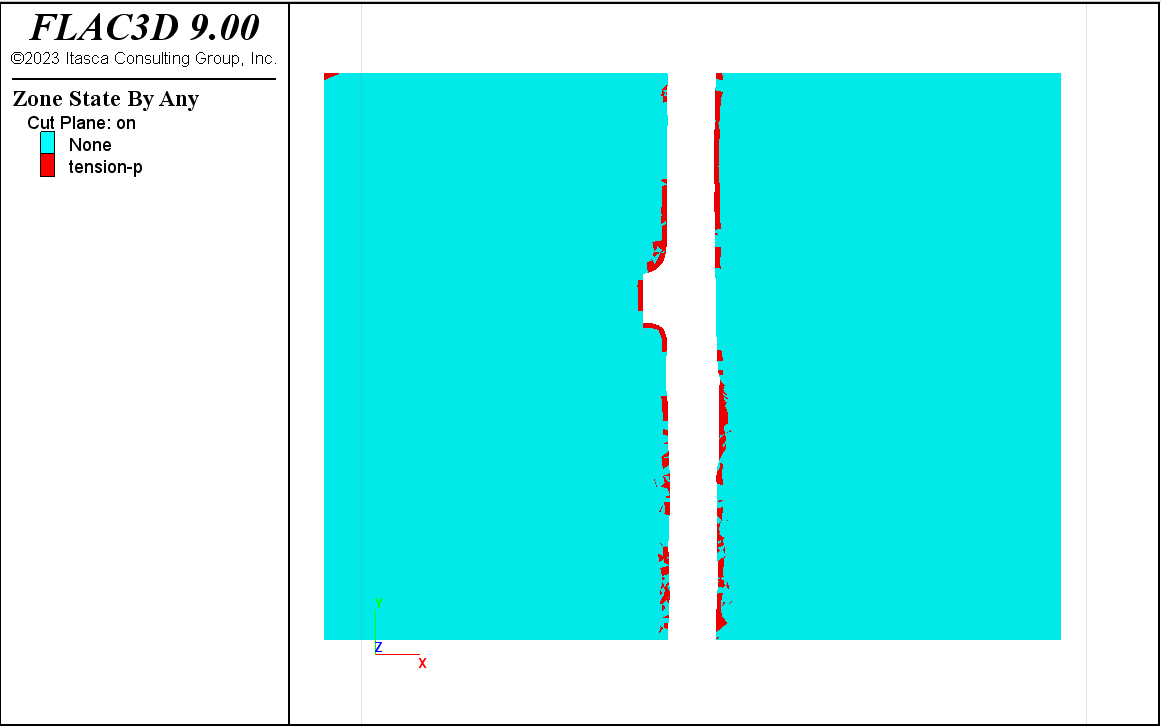
\includegraphics[width=\textwidth]{graphics/plasticity/update1.png}
        \caption{Update 1}
        \label{fig:zk5_1s_mosaic_1}
    \end{subfigure}

    \vspace{1em} % Add some vertical space between rows

    \begin{subfigure}[b]{0.48\textwidth}
        \centering
        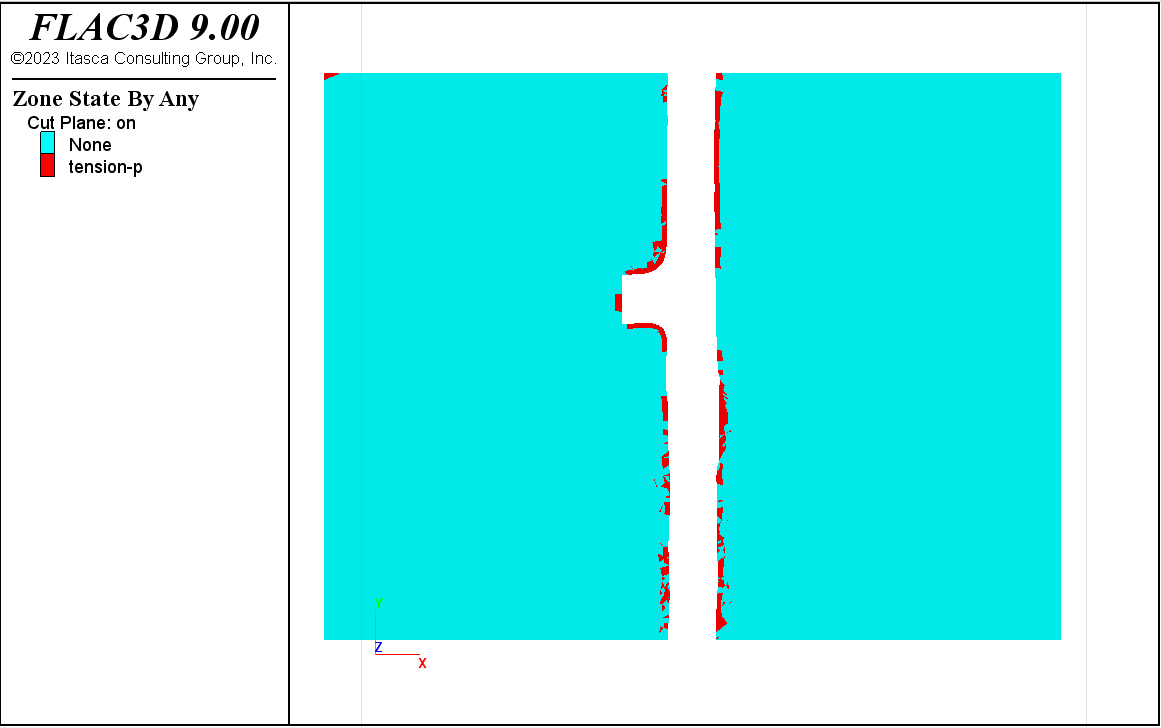
\includegraphics[width=\textwidth]{graphics/plasticity/update2.png}
        \caption{Update 2}
        \label{fig:zk5_1s_mosaic_2}
    \end{subfigure}
    \hfill
    \begin{subfigure}[b]{0.48\textwidth}
        \centering
        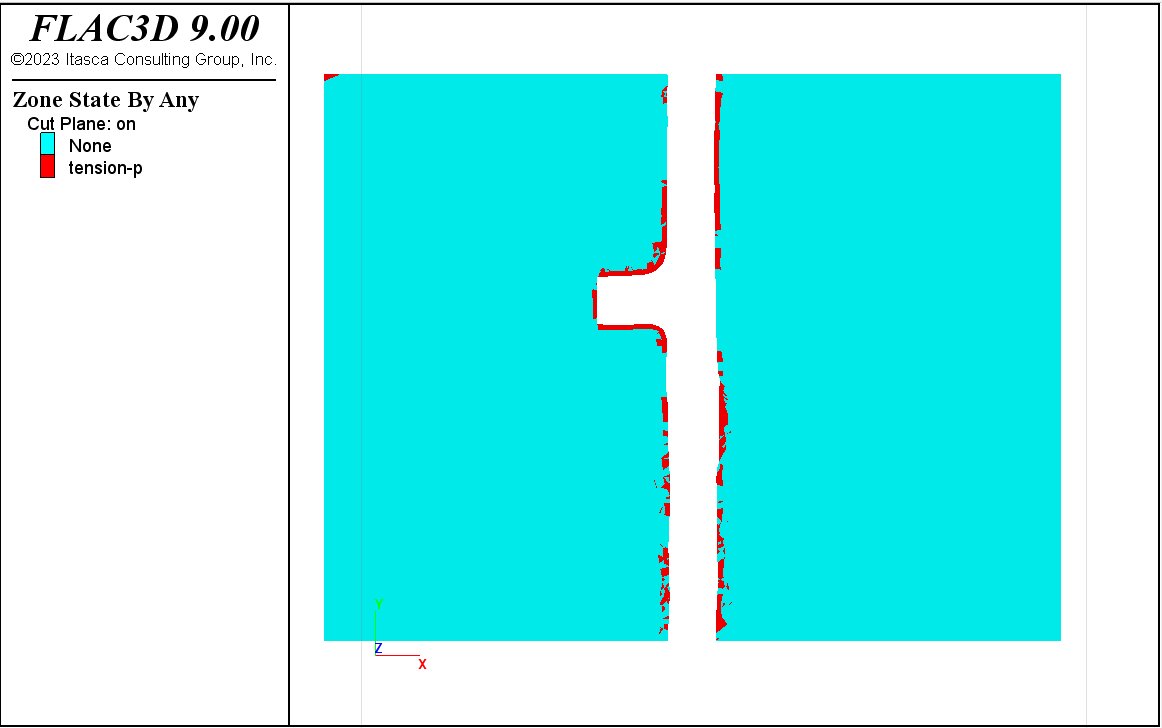
\includegraphics[width=\textwidth]{graphics/plasticity/update3.png}
        \caption{Update 3}
        \label{fig:zk5_1s_mosaic_3}
    \end{subfigure}

    \vspace{1em} % Add some vertical space between rows

    \begin{subfigure}[b]{0.48\textwidth}
        \centering
        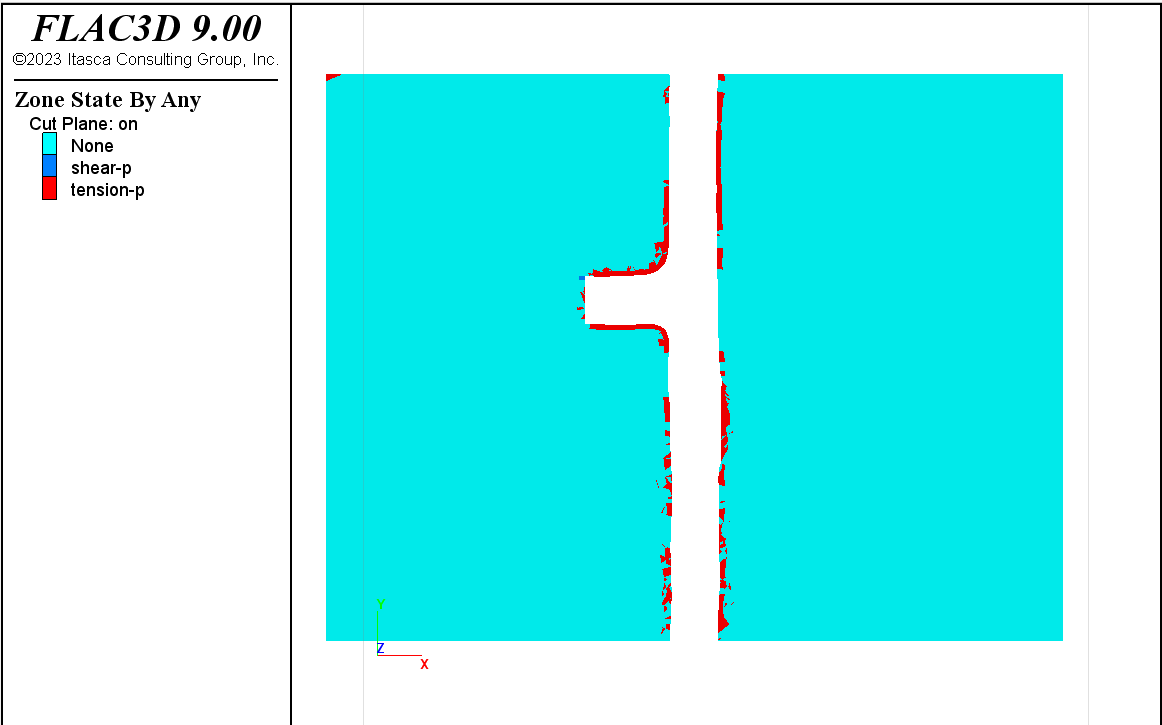
\includegraphics[width=\textwidth]{graphics/plasticity/update4.png}
        \caption{Update 4}
        \label{fig:zk5_1s_mosaic_4}
    \end{subfigure}
    \hfill
    \begin{subfigure}[b]{0.48\textwidth}
        \centering
        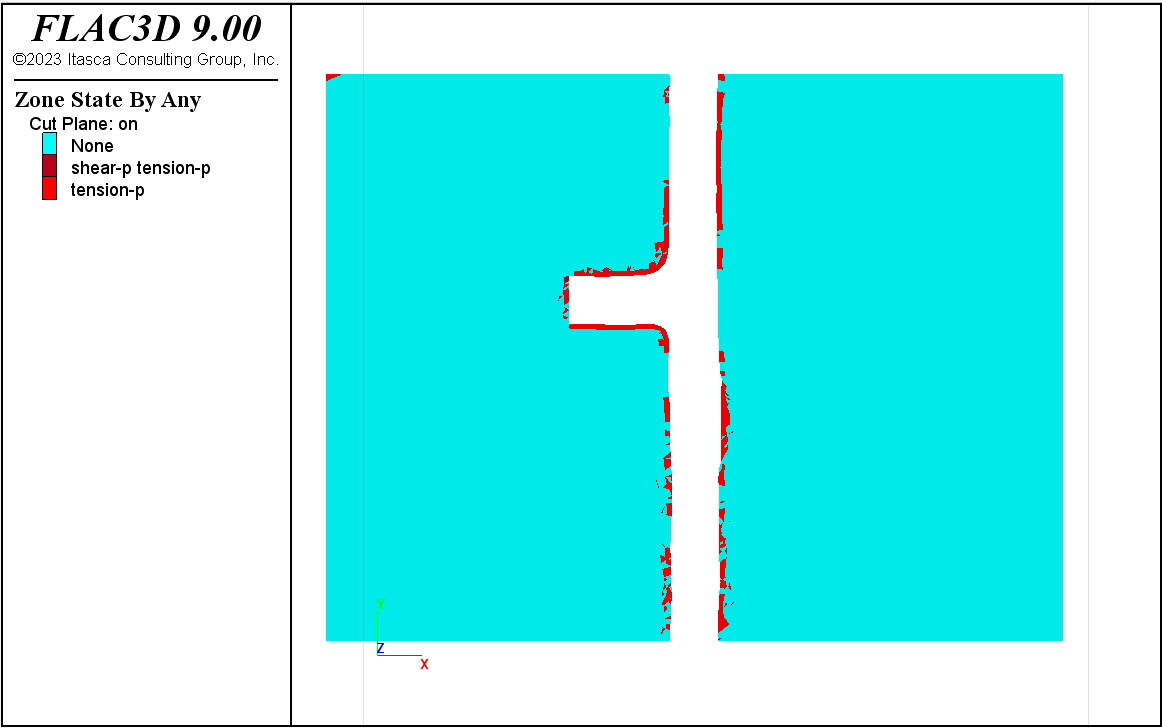
\includegraphics[width=\textwidth]{graphics/plasticity/update5.png}
        \caption{Update 5}
        \label{fig:zk5_1s_mosaic_5}
    \end{subfigure}

    \vspace{1em} % Add some vertical space between rows

    \begin{subfigure}[b]{0.48\textwidth}
        \centering
        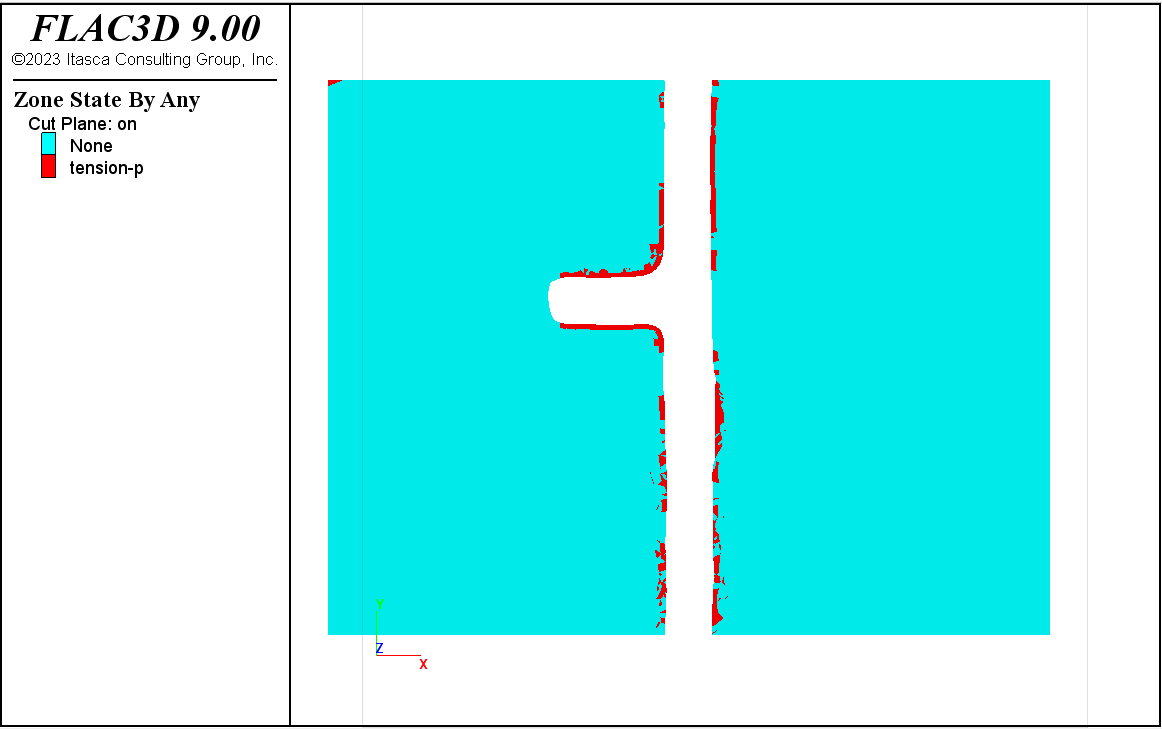
\includegraphics[width=\textwidth]{graphics/plasticity/update6.png}
        \caption{Update 6}
        \label{fig:zk5_1s_mosaic_6}
    \end{subfigure}
    \hfill
    % Add an empty subfigure or filler if you want the last image centered, otherwise it will be left-aligned.
    
    \caption{ZK5-1S Yielded Zones (Zone State By Any) at various excavation updates.}
    \label{fig:zk5_1s_mosaic}
\end{figure}


\begin{figure}%[H]
    \centering
    \begin{subfigure}[b]{0.48\textwidth}
        \centering
        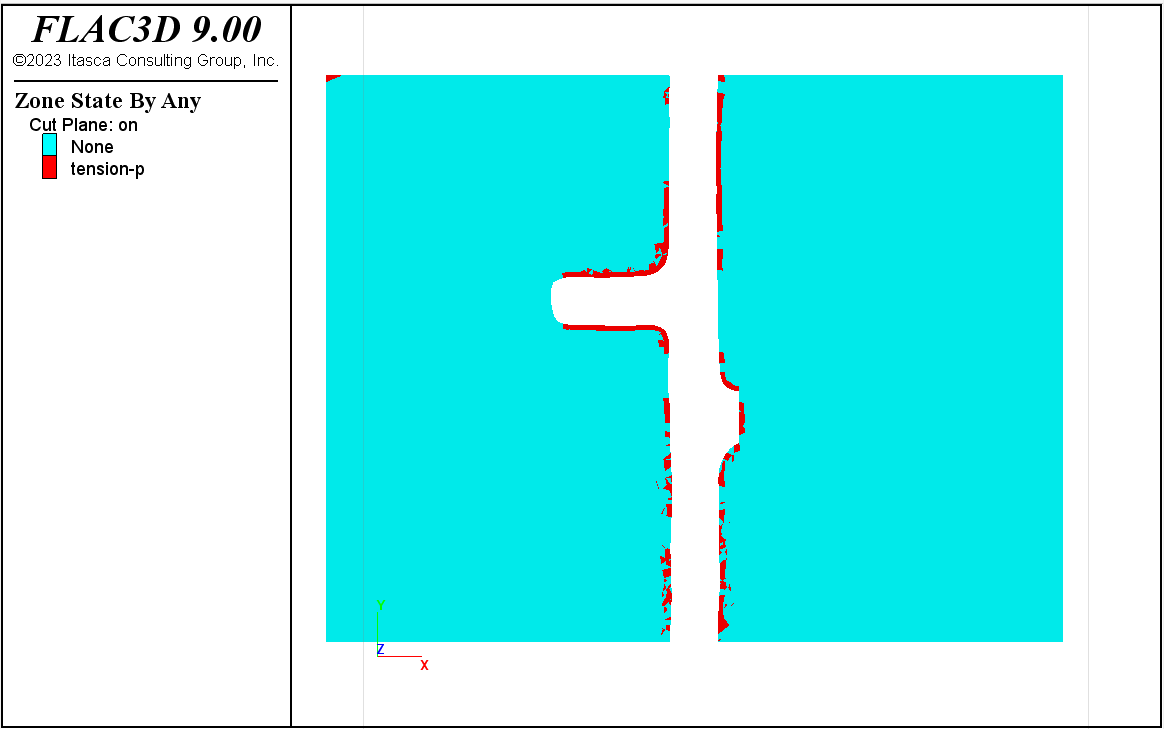
\includegraphics[width=\textwidth]{graphics/plasticity/update7.png}
        \caption{Update 7}
        \label{fig:zk5_1j_mosaic_7}
    \end{subfigure}
    \hfill
    \begin{subfigure}[b]{0.48\textwidth}
        \centering
        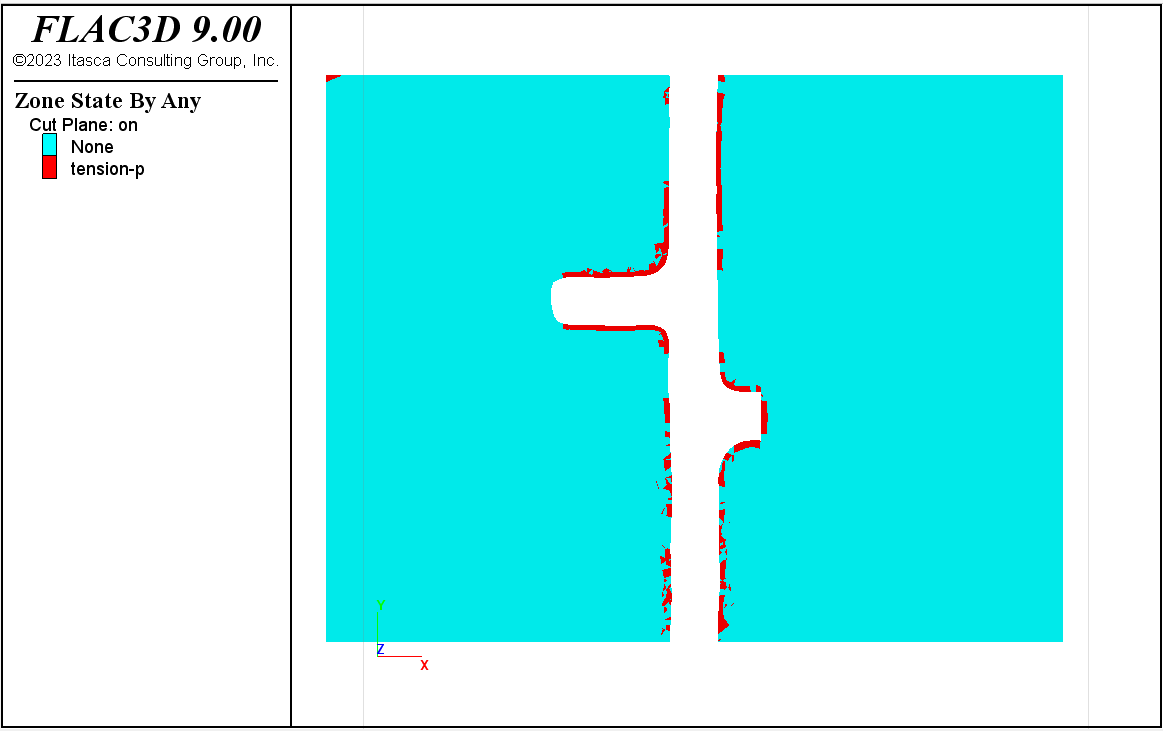
\includegraphics[width=\textwidth]{graphics/plasticity/update8.png}
        \caption{Update 8}
        \label{fig:zk5_1j_mosaic_8}
    \end{subfigure}

    \vspace{1em} % Add some vertical space between rows

    \begin{subfigure}[b]{0.48\textwidth}
        \centering
        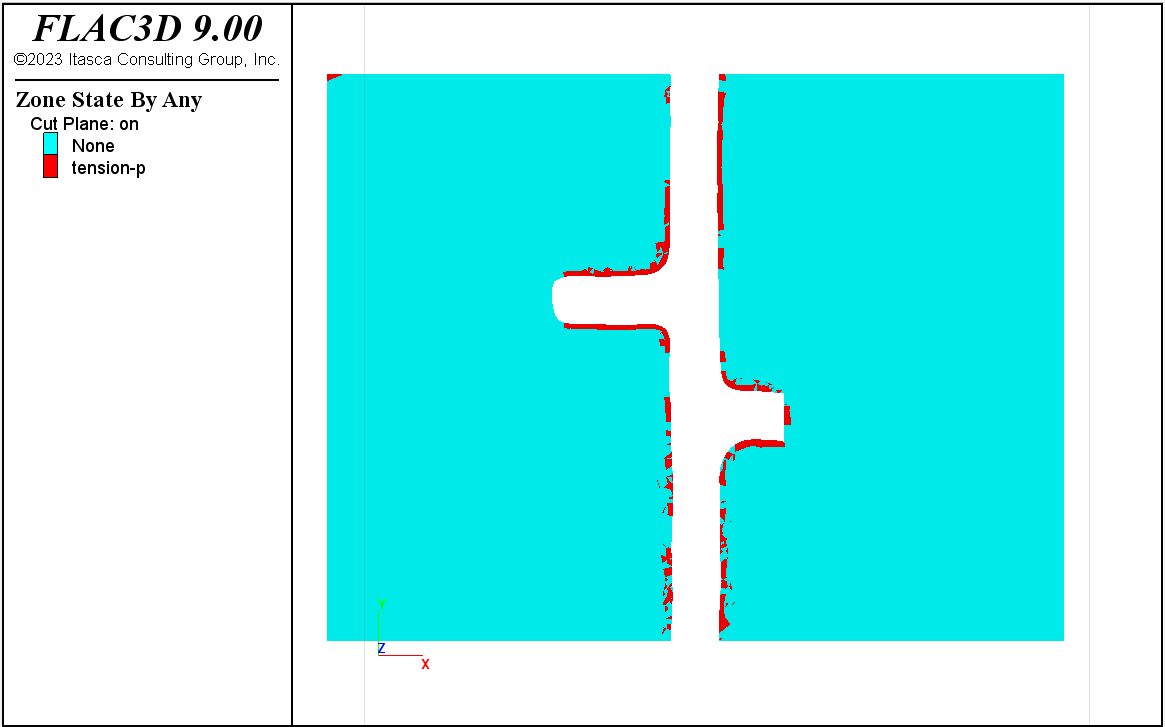
\includegraphics[width=\textwidth]{graphics/plasticity/update9.png}
        \caption{Update 9}
        \label{fig:zk5_1j_mosaic_9}
    \end{subfigure}
    \hfill
    \begin{subfigure}[b]{0.48\textwidth}
        \centering
        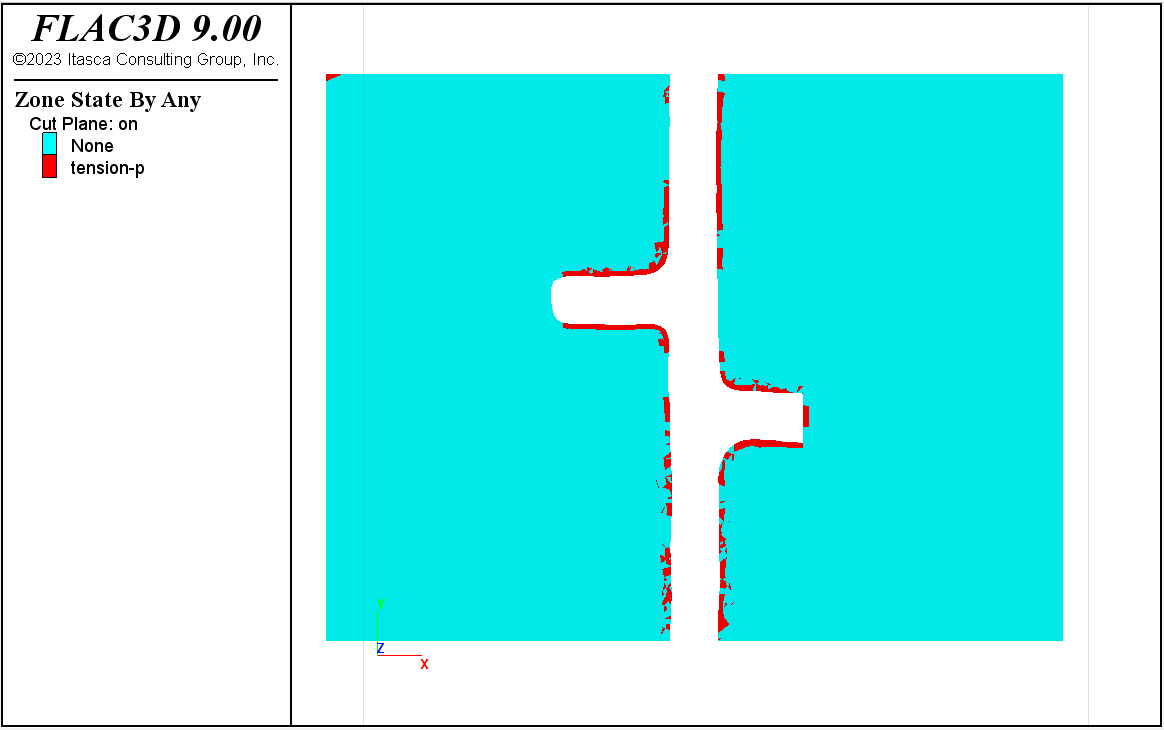
\includegraphics[width=\textwidth]{graphics/plasticity/update10.png}
        \caption{Update 10}
        \label{fig:zk5_1j_mosaic_10}
    \end{subfigure}

    \vspace{1em} % Add some vertical space between rows

    \begin{subfigure}[b]{0.48\textwidth}
        \centering
        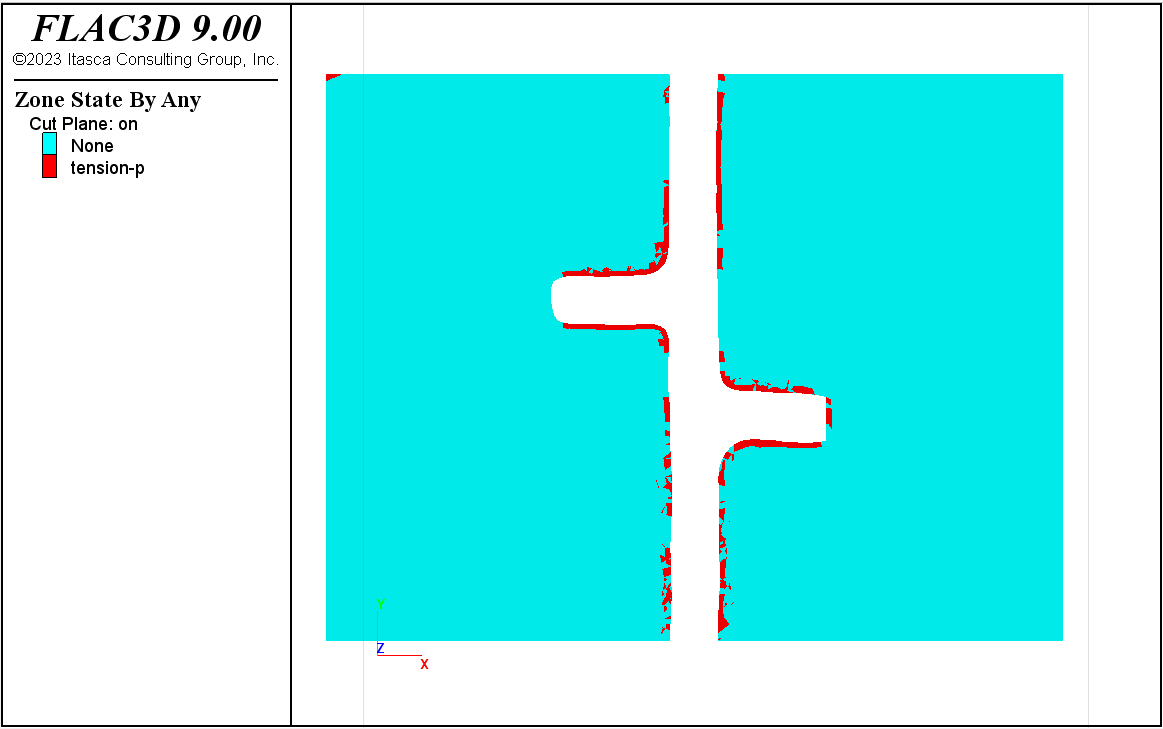
\includegraphics[width=\textwidth]{graphics/plasticity/update11.png}
        \caption{Update 11}
        \label{fig:zk5_1j_mosaic_11}
    \end{subfigure}
    \hfill
    \begin{subfigure}[b]{0.48\textwidth}
        \centering
        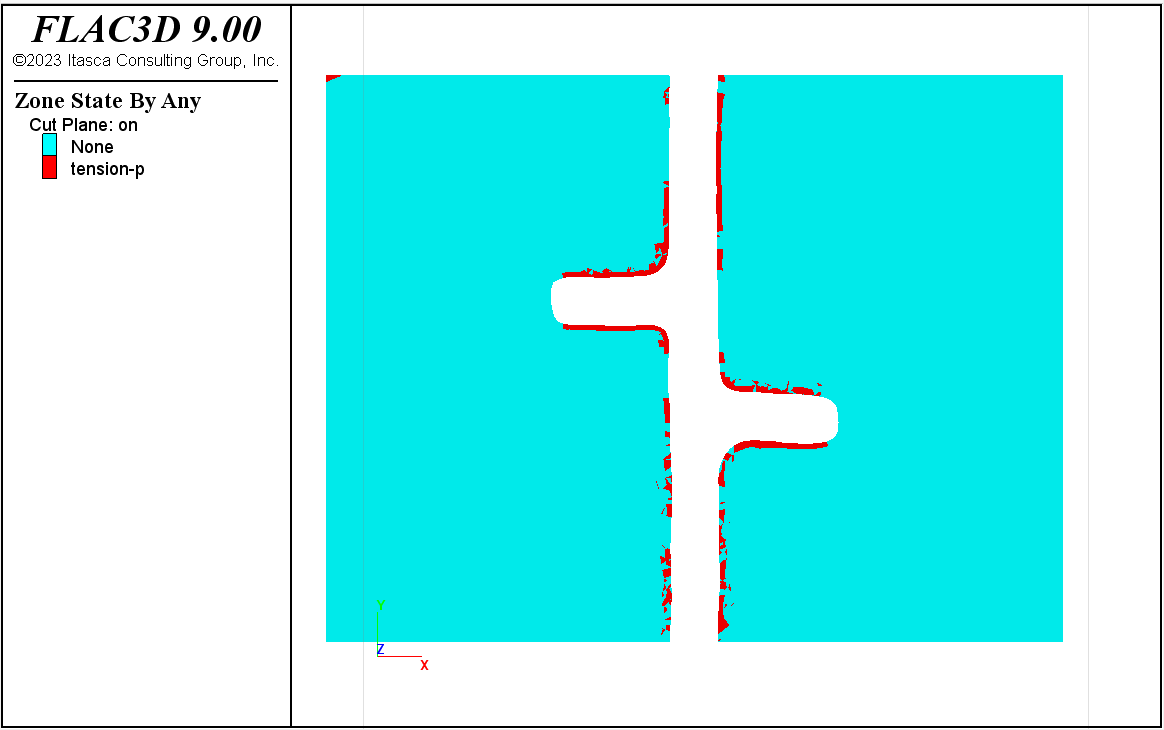
\includegraphics[width=\textwidth]{graphics/plasticity/update12.png}
        \caption{Update 12}
        \label{fig:zk5_1j_mosaic_12}
    \end{subfigure}
    
    \vspace{1em}
    
    \begin{subfigure}[b]{0.48\textwidth}
        \centering
        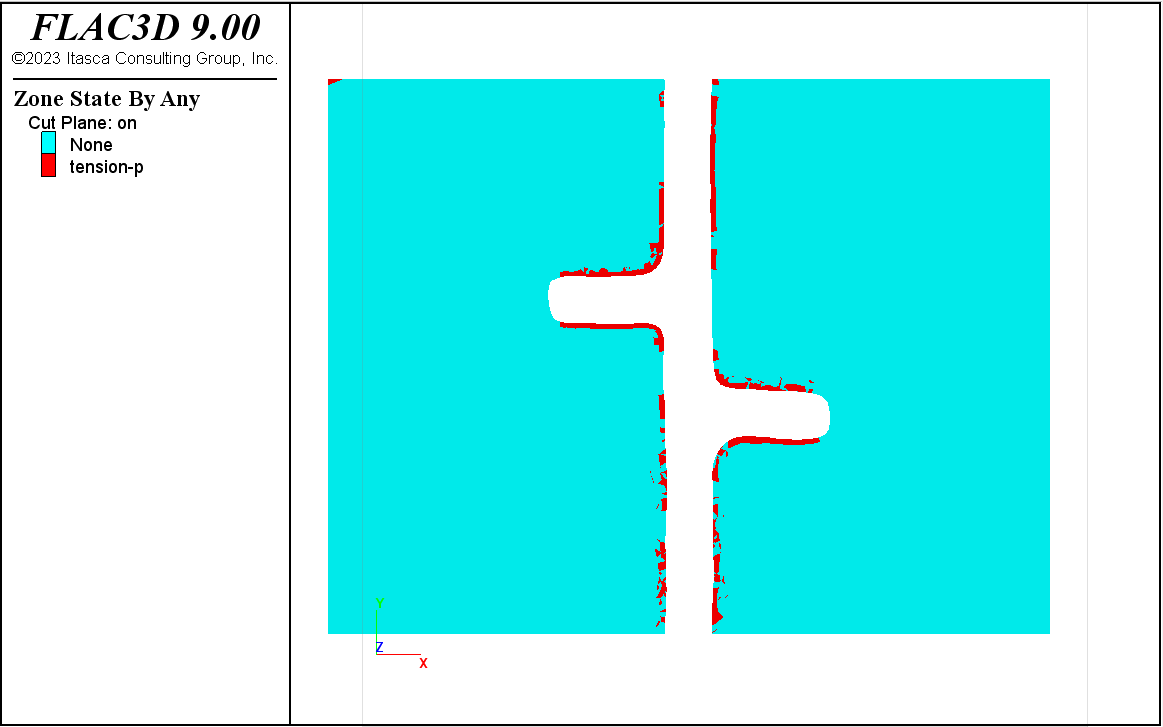
\includegraphics[width=\textwidth]{graphics/plasticity/update13.png}
        \caption{Update 13}
        \label{fig:zk5_1j_mosaic_13}
    \end{subfigure}
    \hfill
    \caption{ZK5-1J Yielded Zones (Zone State By Any) at various excavation updates.}
    \label{fig:zk5_1j_mosaic}
\end{figure}

\subsection{Overall EDZ extent (Update 13)}

\begin{figure}[H]
    \centering
    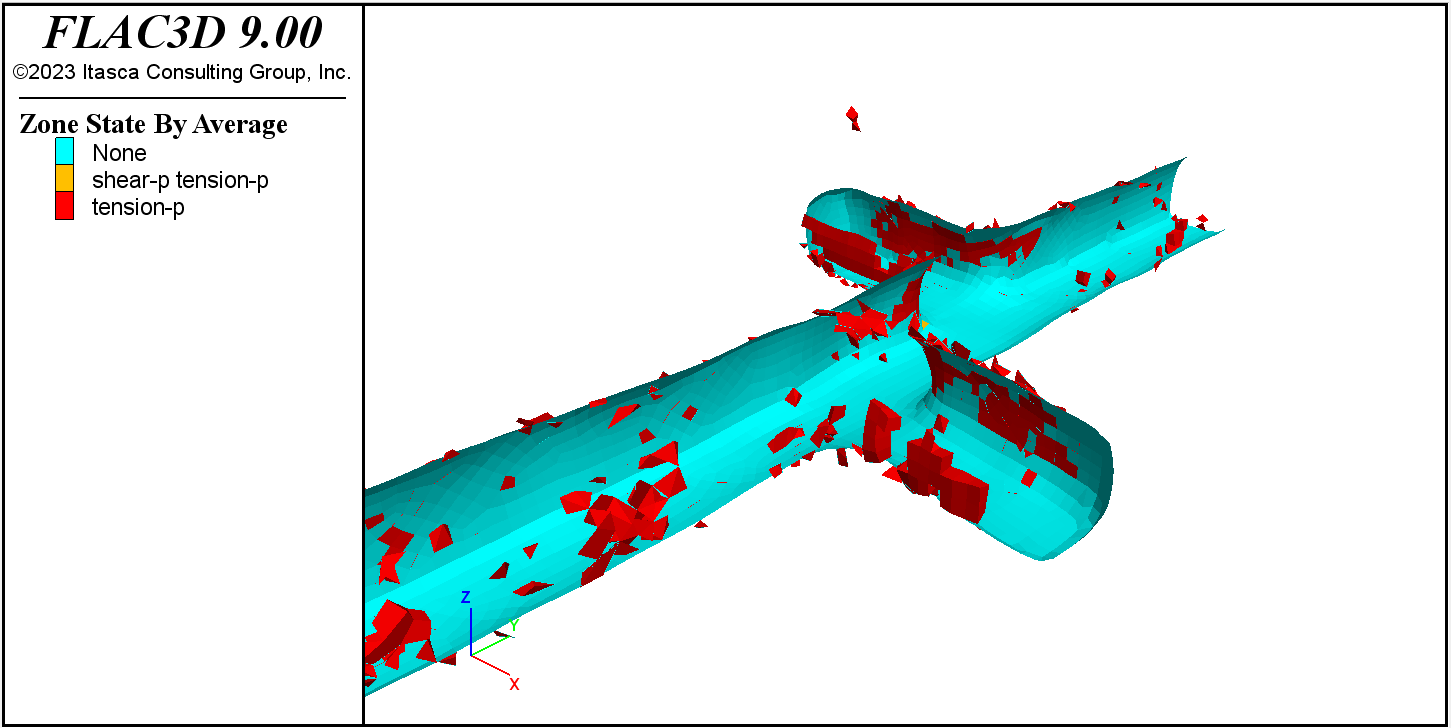
\includegraphics[width=0.9\textwidth]{graphics/plasticity/iso1.png}
    \caption{Update 13 - Zone State By Average (3D view).}
    \label{fig:update13_average}
\end{figure}

\begin{figure}[H]
    \centering
    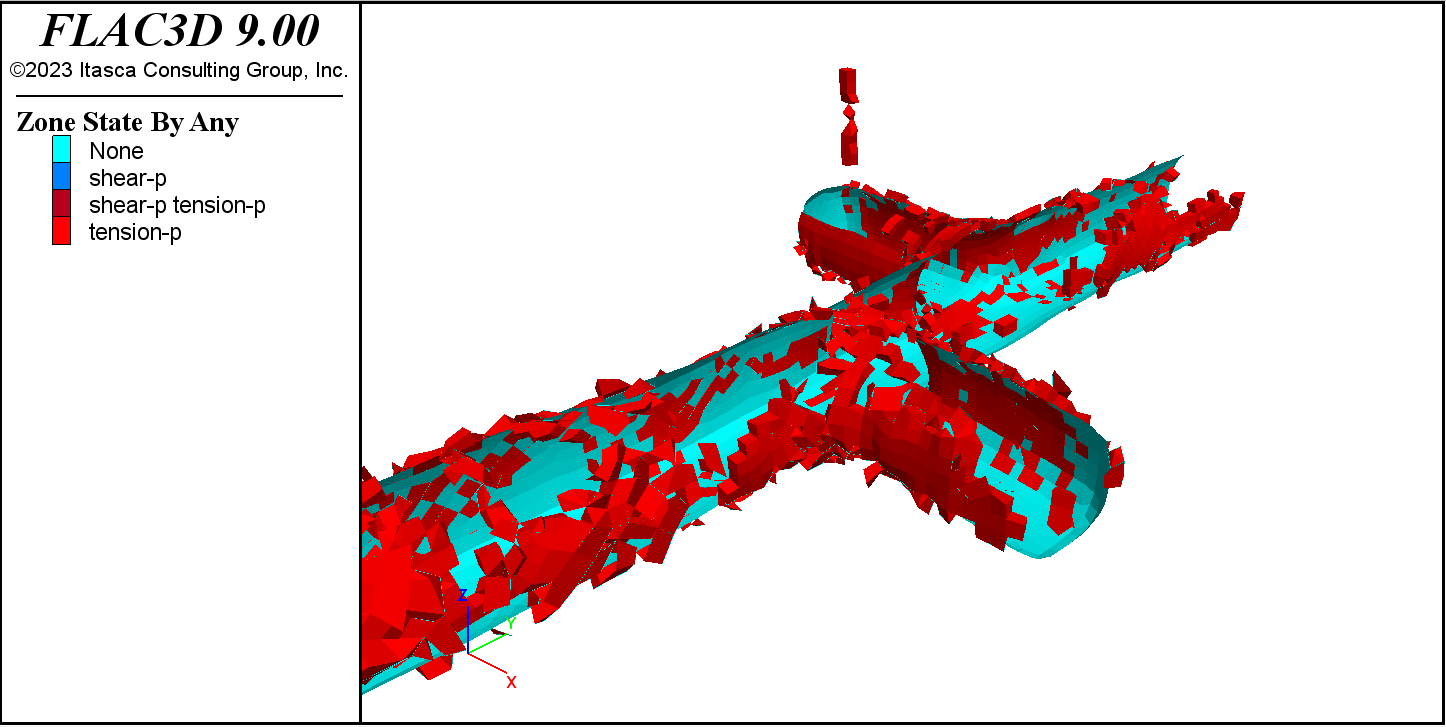
\includegraphics[width=0.9\textwidth]{graphics/plasticity/iso2.png}
    \caption{Update 13 - Zone State By Any (3D view).}
    \label{fig:update13_any}
\end{figure}

\begin{figure}[H]
    \centering
    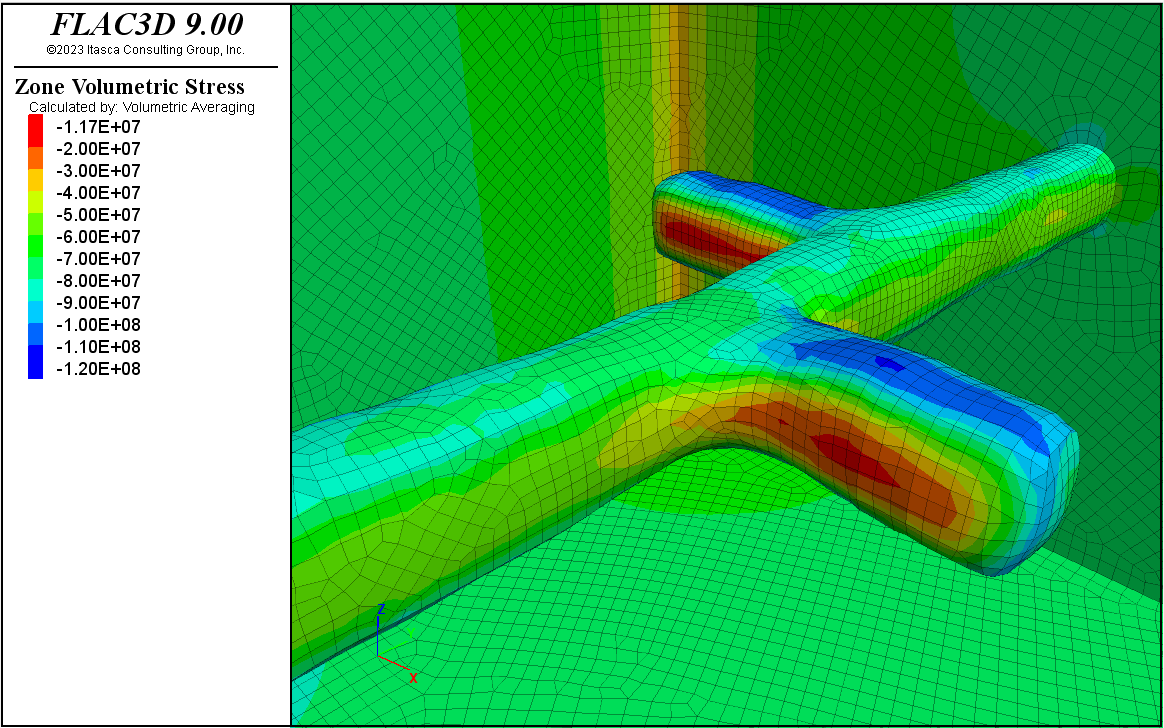
\includegraphics[width=0.9\textwidth]{graphics/plasticity/volumetric.png}
    \caption{Volumetric stress contours at 'update13'.}
    \label{fig:volumetric}
\end{figure}

\begin{figure}[H]
    \centering
    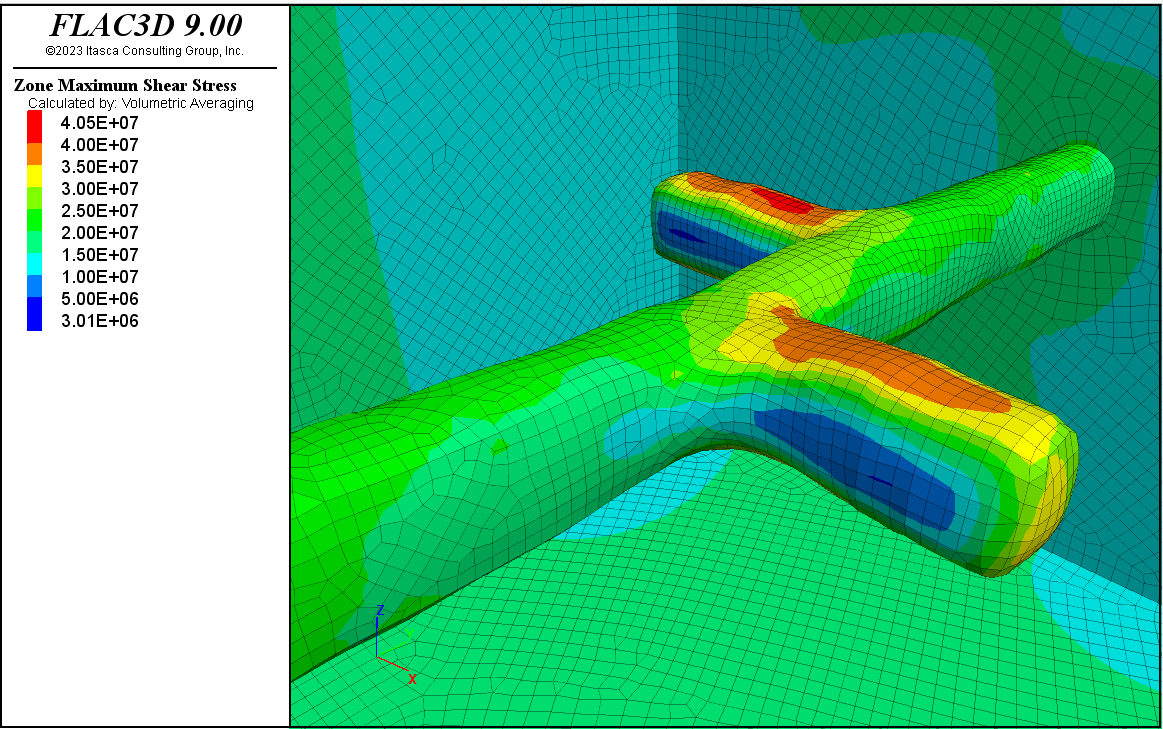
\includegraphics[width=0.9\textwidth]{graphics/plasticity/deviatoric.png}
    \caption{Maximum shear stress contours at 'update13'.}
    \label{fig:shear}
\end{figure}

\begin{figure}[H]
    \centering
    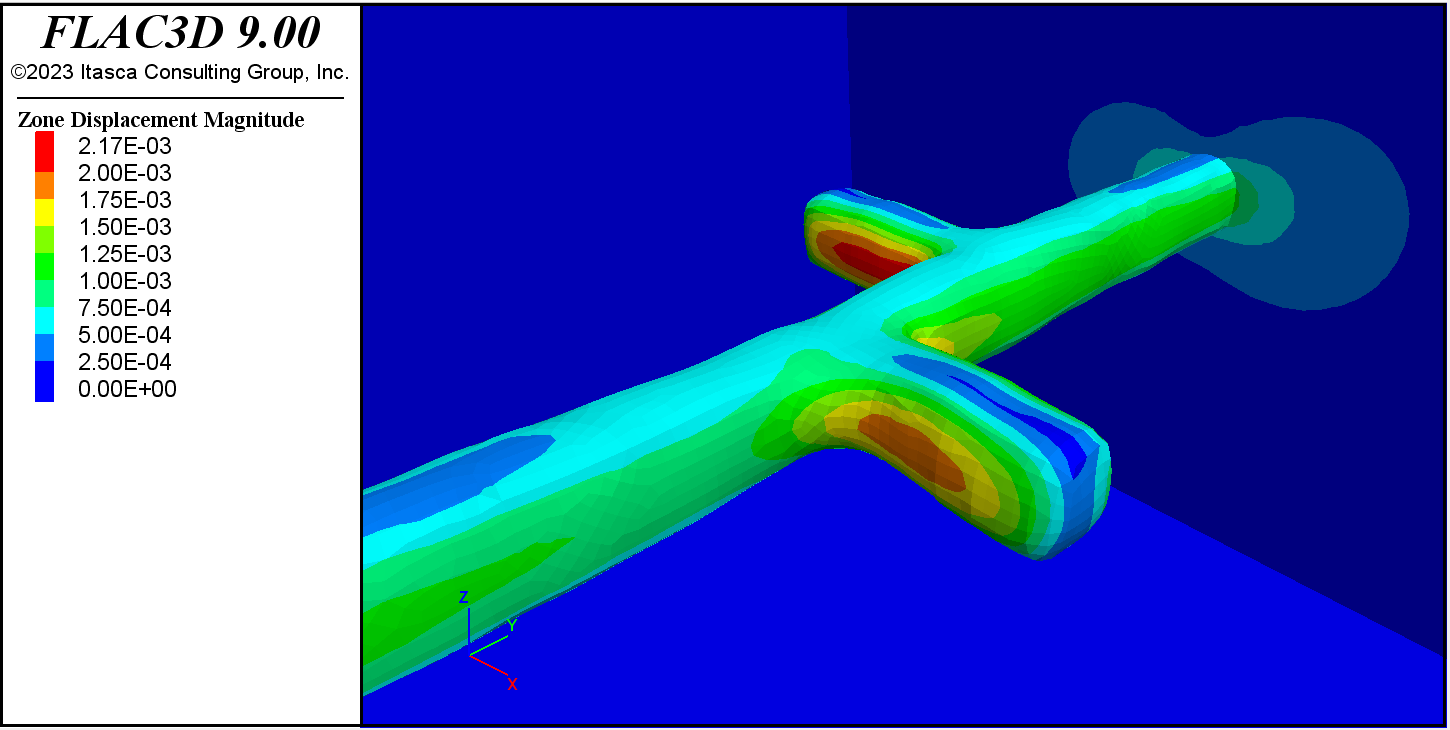
\includegraphics[width=0.9\textwidth]{graphics/plasticity/disp13.png}
    \caption{Displacements at 'update 13'.}
    \label{fig:disp13}
\end{figure}

% \newpage 
\subsection{Discussion}
The visualization of the yielded zones provides clear insight into the development of the \gls{EDZ}. According to \cite{Perras2016} the extent of \gls{EDZ} can be estimated, among other parameters, by yielded elements and principal stress gradients. 
\par The final model state, particularly at the intersections for branches ZK5-1S and ZK5-1J, is especially revealing. The yielded areas, colored red in the 'Zone State By Any' plot (Figure \ref{fig:update13_any}), are not only localized around the tunnel walls but are extensively developed, indicating a significant damage mechanism at play.

\par Crucially, the model's legend clarifies that these red zones represent rock that has failed in tension (tension-p). Therefore, the dominant failure mechanism driving the formation of the \gls{EDZ} is tensile failure. It may seem counterintuitive that such strong rock (UCS = 170.3 MPa, GSI = 88) would exhibit a notable damage zone, but high-strength crystalline rocks such as amphibolite are very brittle. Although they are exceptionally strong in compression, they are notoriously weak in tension, with tensile strengths on the order of typically only $5-10~\%$ of the UCS (\cite{Cai2010}).

The Volumetric Stress plot (Figure \ref{fig:volumetric}) illustrates this process perfectly; while high compressive stresses (blue/green contours) wrap around the tunnel, the sharp corners of the intersections, especially at branch ZK5-1J create zones of low confinement and induced tension (red/yellow contours). As rock is significantly weaker in tension than in compression, it fails in this \textquote{weakest link} mode first. The high competence of the rock means that once this tensile limit is breached, failure (spalling, fracturing) initiates readily and can propagate. The high competence of the rock means that once this tensile limit is breached, failure (spalling, fracturing) initiates readily and can propagate, a process well-documented in brittle rocks like granite (\cite{Martin1994,Perras2016}). The model captures this clearly.

\par This tension-driven damage pattern is powerfully explained by a key observation: displacements on the roof and floor are an order of magnitude less than on the walls. This highlights the rock's response to a highly anisotropic in-situ stress field, likely with the major principal stress acting horizontally. The model, even with a simplified isotropic Hoek-Brown material, correctly captures how this horizontal stress concentration on the walls induces the tensile stresses responsible for the extensive tension-yielded zones.

\par The model demonstrates a strong, self-consistent correlation between all the outputs, validating its ability to capture this localized, tension-driven damage mechanism. The regions of most extensive tensile failure (Figure \ref{fig:update13_any}) correspond directly to:
\begin{enumerate}
    

\item The zones of lowest volumetric (compressive) stress in Figure \ref{fig:volumetric}.

\item The areas of highest maximum shear stress in Figure \ref{fig:shear}, though the rock fails in tension before reaching its full shear strength limit.

\item The locations of the largest displacement magnitudes (up to \num{2.17E-03}) in Figure \ref{fig:disp13}.\end{enumerate}

For a practical engineering assessment, the comparison between the detailed 'Zone State By Any' plot and the more conservative 'Zone State By Average' is essential. Therefore, the true extent of the damage lies somewhere between these two visualizations, providing a robust range for the estimated \gls{EDZ} width of 0.5 m to 1 m. Figure \ref{fig:disp13} offers a final visual summary, powerfully reinforcing that the largest ground deformations are a direct consequence of the widespread tensile failure within the \gls{EDZ}.
% \newpage


\subsection{Influence of EDZ on the hydraulic conductivity}

The results obtained with the Hoek–Brown model were further compared with the linear elastic case in order to assess the impact of material nonlinearity.
Figure~\ref{fig:stress_el_hb} shows that, in the linear elastic case, the stress magnitude reaches approximately $\SI{110}{\MPa}$.
The region where the stress predicted by the linear elastic and Hoek–Brown models differs by more than $\SI{1}{\MPa}$ is confined to a zone extending approximately one to two mesh elements from the excavations, i.e. within the \gls{EDZ}.
In the remainder of the computational domain, the stress fields are almost identical.

\begin{figure}
    \centering
    \begin{subfigure}{\textwidth}
        \centering
        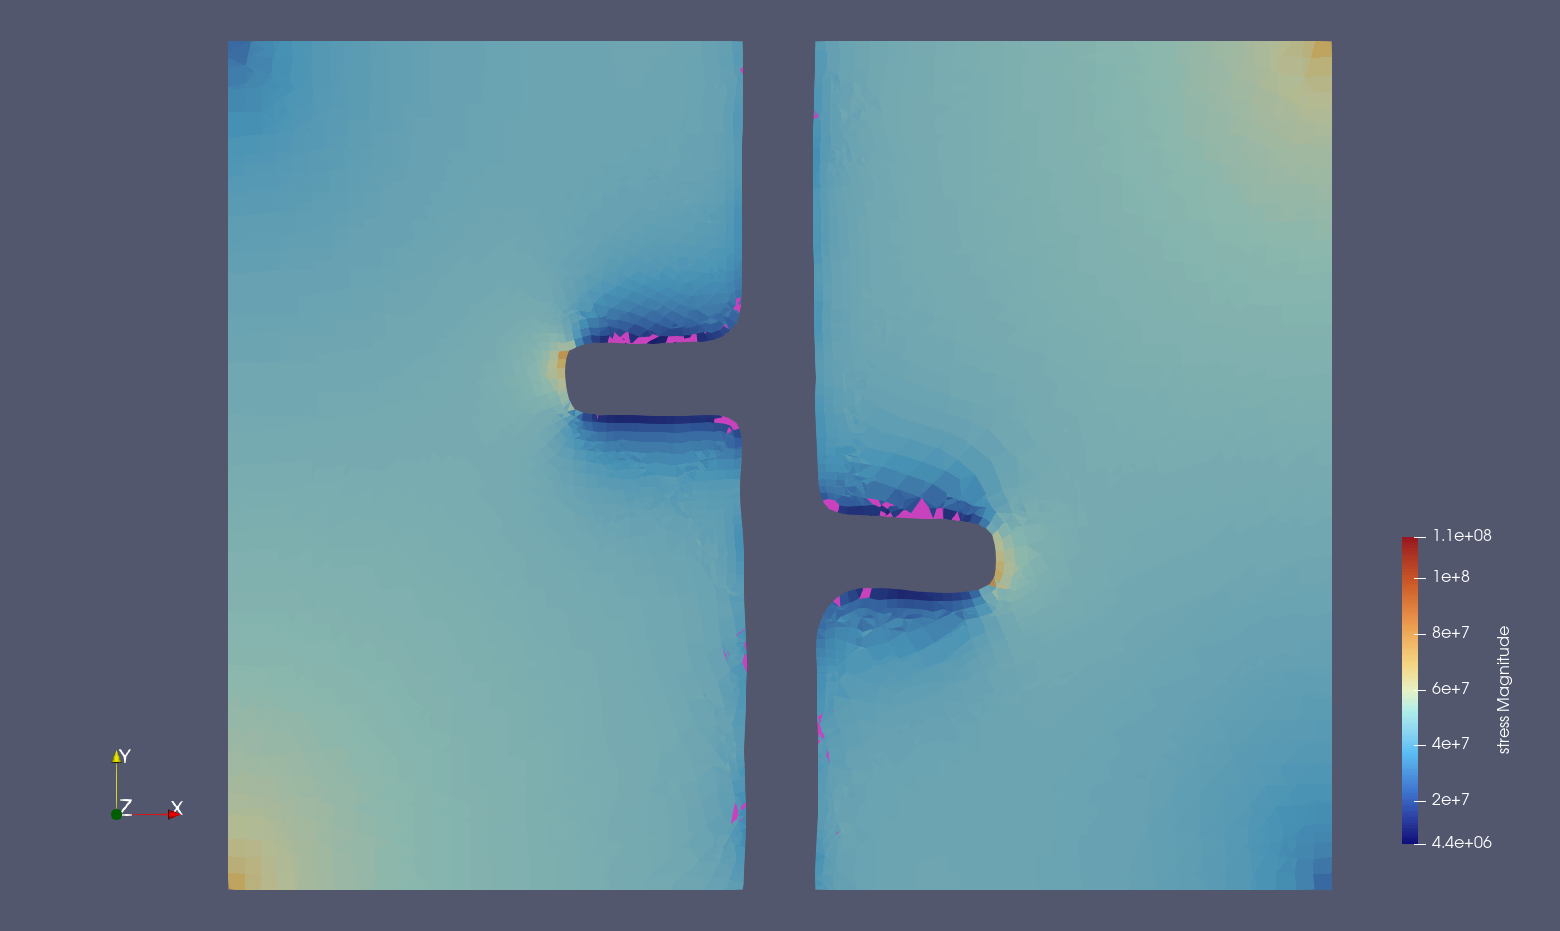
\includegraphics[width=0.75\textwidth]{graphics/comparison/stress_diff.png}
        \caption{Stress magnitude obtained with the linear elastic model. Areas highlighted in pink indicate regions where the stress difference between the linear elastic and Hoek–Brown models exceeds $\SI{1}{\MPa}$.}\label{fig:stress_el_hb}
    \end{subfigure}
    \begin{subfigure}{\textwidth}
        \centering
        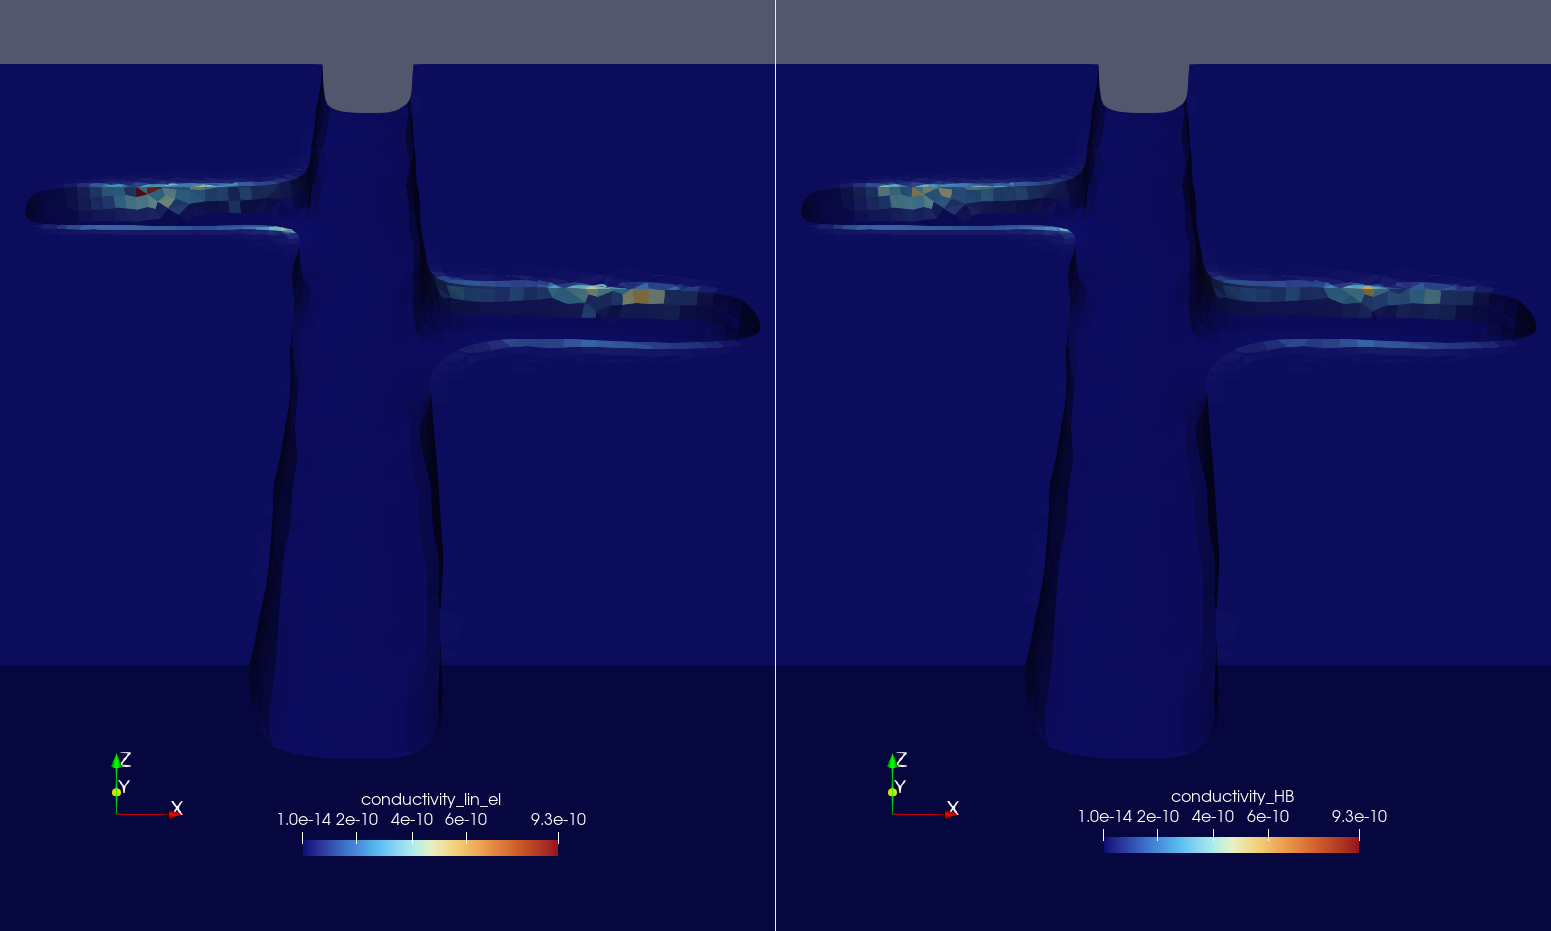
\includegraphics[width=0.75\textwidth]{graphics/comparison/cond_diff.png}
        \caption{Hydraulic conductivity derived from the stress field. Left: linear elastic model; right: Hoek–Brown model.}\label{fig:cond_el_hb}
    \end{subfigure}
    \caption{Comparison of the linear elastic and Hoek-Brown constitutive models.}
\end{figure}

As the stress differences are confined to a narrow layer around the excavations, a natural question arises as to how the computed hydraulic conductivity is affected by the choice of the mechanical model.
Figure~\ref{fig:cond_el_hb} shows the hydraulic conductivity computed using the relation given in Eq.~\eqref{eq:conductivity_relation} for both constitutive models.
Significant differences are again observed only within the \gls{EDZ}.
In the linear elastic case, the hydraulic conductivity reaches $\SI{9.3e-10}{\mps}$, whereas for the Hoek–Brown model the maximum value is $\SI{5.7e-10}{\mps}$, i.e. approximately $30~\%$ lower.
Consequently, over most of the computational domain the linear elastic constitutive model provides sufficiently accurate results, while within the \gls{EDZ} it leads to a slight overestimation of the hydraulic conductivity.


\subsection{Summary}
In this section, the implementation of a Hoek-Brown model within FLAC3D was presented, that was used to assess the \gls{EDZ} at the \URFBII. The key findings and conclusions are as follows:
\begin{enumerate}
\item \textbf{Model Simplification and Geotechnical Parameters:} The numerical model was effectively simplified to a single Hoek-Brown material with properties characteristic of the dominant amphibolite lithology (E=72.5 GPa, $\nu$=0.215, UCS=170.3 MPa). This focused approach proved highly effective, demonstrating that a simplified model can capture complex, stress-path-dependent geotechnical behavior. Crucially, it successfully simulated the development of a tension-dominated \gls{EDZ} in response to an inferred anisotropic stress field, demonstrating its predictive power.

\item \textbf{Mesh Generation and Refinement:} The successful refinement of the initial scanned mesh using Rhino commands (e.g., QuadRemesh) was a critical prerequisite for the analysis. This process eliminated artifacts and produced a high-quality, hexahedral-dominant mesh, enabling a precise simulation of the stress concentrations and failure mechanisms at the complex tunnel intersections.

\item \textbf{Pore Pressure Simulation and Interpolation:} The robust script for importing and interpolating pore pressure data functioned flawlessly. The use of a Gaussian filter ensured a smooth and realistic pore pressure field, establishing a reliable effective stress framework, which is fundamental for accurately predicting rock mass failure.

\item \textbf{EDZ Characterization and Failure Mechanism:} The primary conclusion of this study is that the \gls{EDZ} is predominantly driven by tensile failure. 
\par This is a direct response to a highly anisotropic in-situ stress field, evidenced by wall displacements being an order of magnitude larger than those in the roof and floor. This stress condition induces tensile zones on the tunnel walls, where the rock fails according to its \textquote{weakest link}: its low tensile strength. This tension-driven damage is most severe at the tunnel intersections, particularly at branch ZK5-1J, where geometric stress concentrations are highest. The estimated radial extent of the \gls{EDZ} is approximately 0.5 m, extending up to 1 m in these highly stressed intersection zones. This range is robustly defined by comparing the Zone State By Any and Zone State By Average visualizations. The strong correlation between the locations of tensile failure, low volumetric stress, and maximum displacement confirms the model's validity and provides a comprehensive understanding of the tunnel's geomechanical behavior. \end{enumerate}

Finally, the analysis successfully demonstrates that even in a highly competent and strong rock mass, a significant \gls{EDZ} can develop if the in-situ stress field is sufficiently anisotropic, with the failure being driven by the rock's low tensile strength rather than its high compressive strength. The consistency across all presented figures provides a high degree of confidence in the conclusions.




\section{Chapter summary}

We presented two models of mechanical response to excavation and pore pressure changes.
The models were built using two simulation software packages covering different physical aspects (coupled poroelasticity vs. plasticity).
The mechanical parameters of the models were successfully harmonized to give comparable results in the linear elastic regime.

The study of \Gls{EDZ} extent based on the Hoek-Brown plasticity model revealed a robust estimate for the \Gls{EDZ} width of $0.5-1$ \unit\meter, with the damage being caused predominantly by the rock's low tensile strength.
In this zone the poroelastic approximation overestimates the stress field and hydraulic conductivity, compared to the Hoek-Brown plasticity model. On the other hand, at larger distance from the excavations, both models yield almost identical values of displacement and stress, meaning that the poroelasticity still gives a meaningful and conservative estimate of the disturbed rock permeability.

